\newcommand{\AWSSTS}{Serviciu web ce permite unui utilizator sa solicite credentiale temporare pentru autentificarea in cadrul platformei Amazon Web Services}
\newcommand{\openIDDefinition}{http://openid.net/what-is-openid/}

\usemintedstyle{rrt}

Esenta aplicatiei "Surf" se afla in codul executat de serviciul web AWS Lambda, care preia componentele dezvoltate pentru crawling web si le executa drept programe autonome folosind infrastructura AWS. AWS Lambda executa acest cod doar cand este nevoie (e.g. la cererea utilizatorului care doreste sa demareze operatiunea de crawling). Se minimizeaza, astfel, atat costurile utilizatorului in ceea ce priveste rularea crawler-ului web (nu necesita hardware dedicat pentru procesarea paginilor web), cat si costurile dezvoltatorilor crawler-ului, care nu trebuie sa rezerve hardware in cloud (e.g. masini virtuale Amazon EC2, inchiriere de hosturi), ca mai apoi, cand nu exista cereri suficiente, aceste masini de calcul sa ramana nefolosite. De asemenea, se renunta la necesitatea de a avea un load-balancer care sa distribuie sarcinile de crawling pe capacitatea hardware disponibila, deoarece acest lucru este administrat, in fundal, de catre AWS Lambda.
\\
\\
Functiile programatice disponibile prin serviciul AWS Lambda pot fi accesate de catre utilizatori printr-un API Restful gazduit de AWS API Gateway. Aceasta platforma permite integrarea cererilor HTTP externe cu mecanismul de autentificare si autorizare a utilizatorilor si codul executat de instantele functiilor Lambda. De asemenea, aplicatia utilizeaza functionalitati de management, monitorizare si analiza a traficului din cadrul API-ului "Surf" care permit, printre altele, inregistrarea si monetizarea functionalitatilor oferite de serviciul web pentru fiecare utilizator in parte. 
\\
\\
Pentru a putea accesa functionalitatile oferite de API-ul "Surf", utilizatorii trebuie sa se autentifice cu un furnizor tert de identitati ce suporta OpenID\footnote{\openIDDefinition}. Credentialele obtinute sunt impachetate intr-o cerere catre AWS Security Token Service\footnote{\AWSSTS}, unde sunt validate. In cazul in care validarea este indeplinita cu succes, Security Token Service returneaza utilizatorului credentiale temporare pentru a accesa servicii din cadrul AWS. Utilizatorul trebuie sa includa aceste credentiale in fiecare cerere catre API-ul "Surf" (autentificare). Odata autentificat, utilizatorul poate interactiona doar cu acele resurse ale API-ului pentru care are drepturi de acces. 
\newpage

\begin{figure}[ht]
\begin{center}
	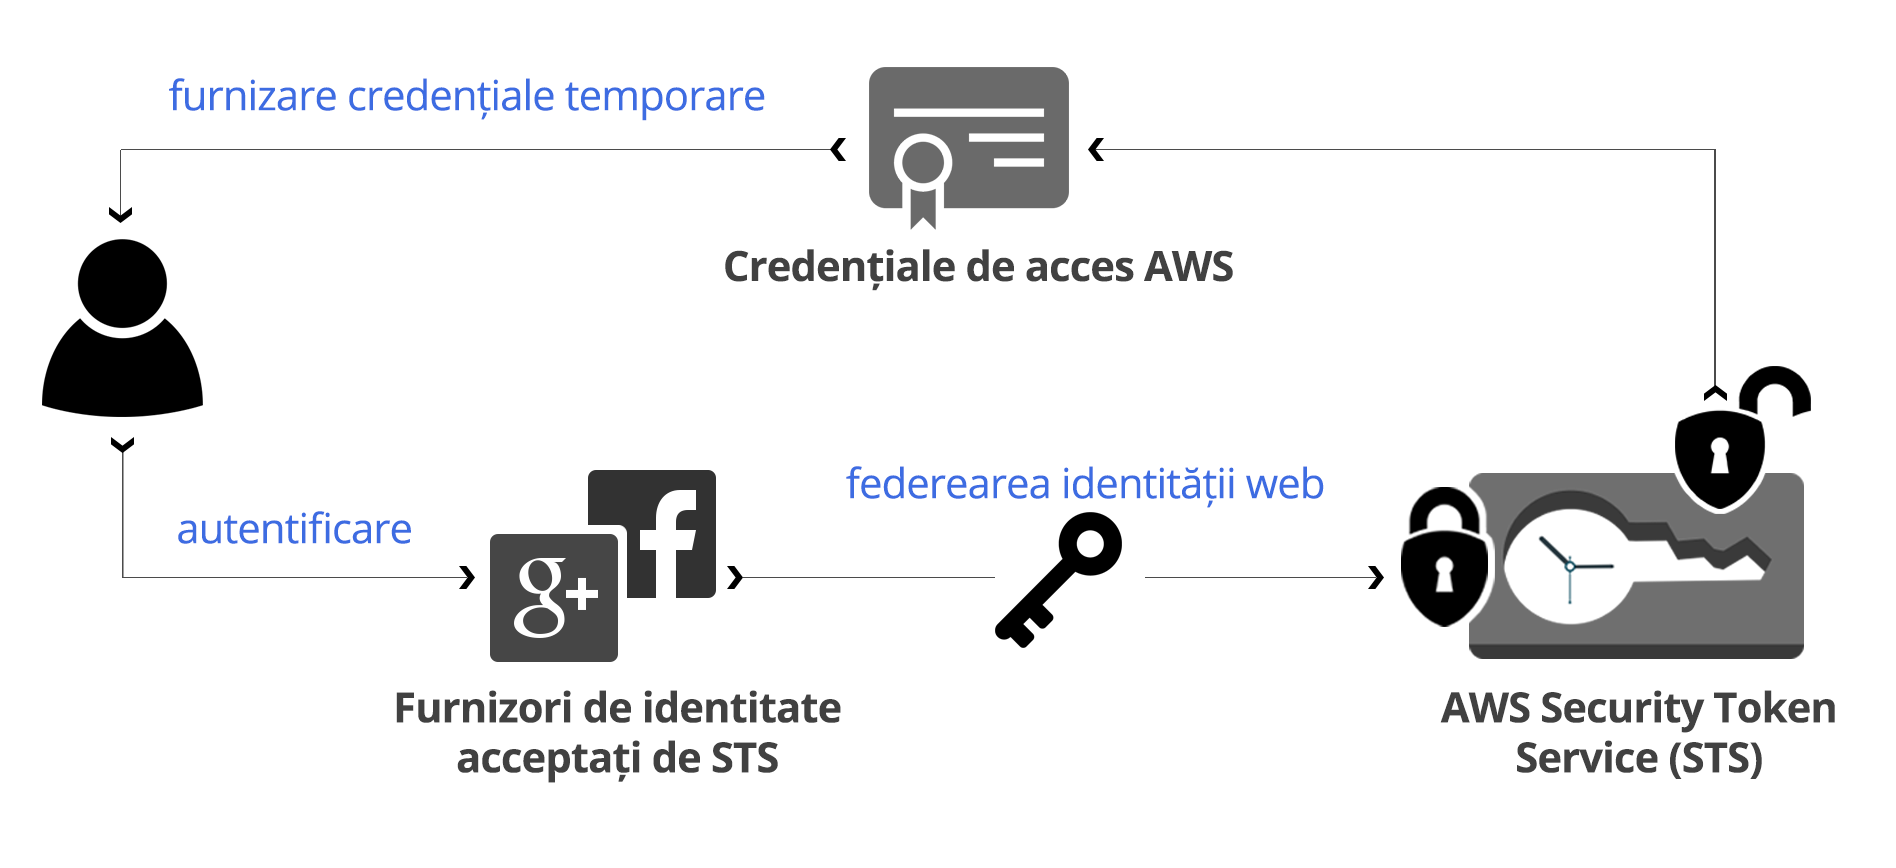
\includegraphics[keepaspectratio, width=1.0\textwidth]{obtinere-credentiale-aws.png}
	\caption{Procesul de autentificare \cite{diagram-icons-sources}}\par\medskip
	\vspace{10mm}
	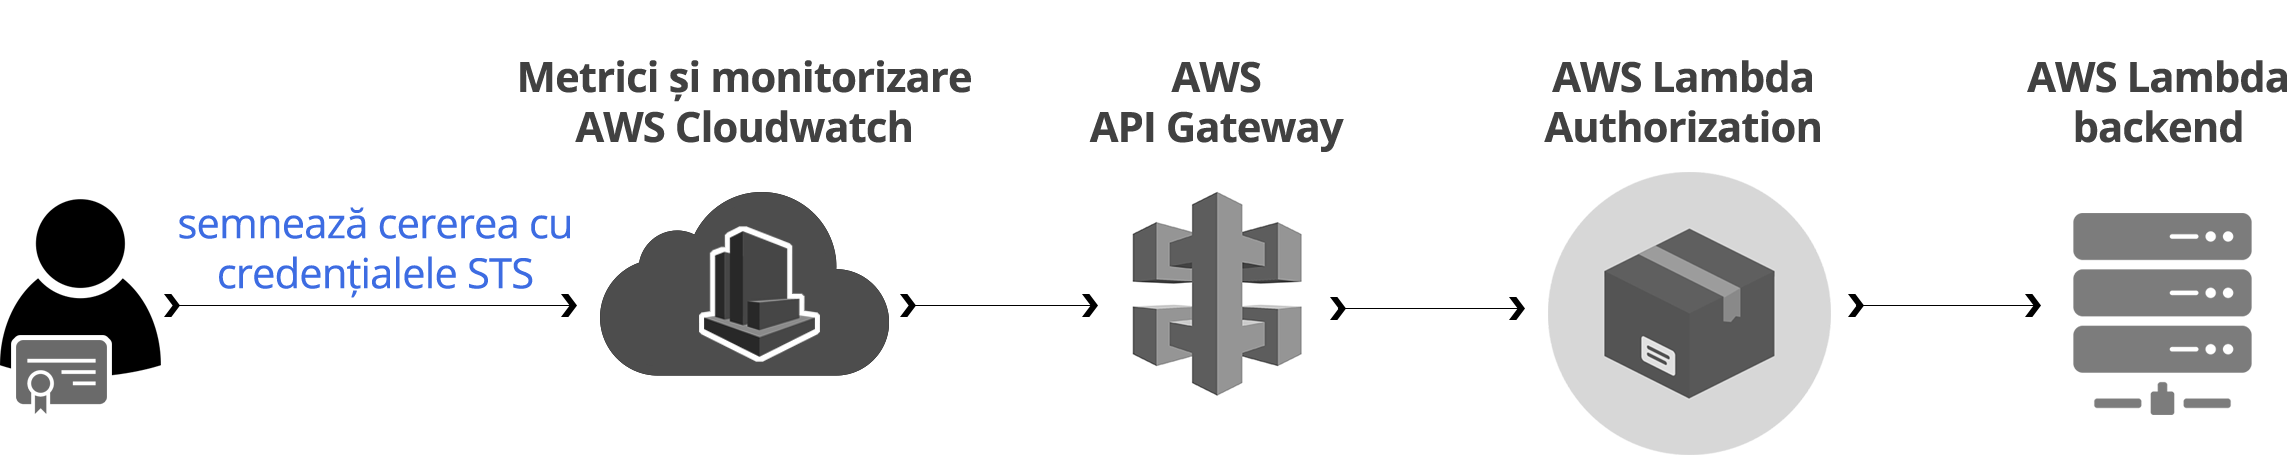
\includegraphics[keepaspectratio, width=1.0\textwidth]{autorizare.png}
	\caption{Procesul de autorizare \cite{diagram-icons-sources}}\par\medskip

\end{center}
\end{figure}

\noindent
Prin AWS Identity Access Management (IAM) se vor stabili restrictiile de acces asupra API-ului. Mecanismul de asignare a permisiunilor va fi sustinut prin definirea unor roluri. Utilizatorii vor fi grupati, din punct de vedere al drepturilor de acces, in mai multe categorii. Spre exemplu, un utilizator poate avea rolul "administrator" (prescurtat \emph{Ad}), iar un alt utilizator poate avea atat rolul "administrator" (\emph{Ad}) cat si "utilizator de baza" (prescurtat \emph{Ub}). Atat \emph{Ad}, cat si \emph{Ub} vor avea asignate politici de acces asupra datelor AWS. O astfel de politica este urmatoarea:
\newpage

\begin{figure}[ht]
\begin{minted}{json}
{
  "Version": "2012-10-17",
  "Statement": [
    {
      "Effect": "Allow",
      "Action": [
        "apigateway:*"
      ],
      "Resource": [
        "*"
      ]
    }
  ]
}
\end{minted}
\begin{center}
	\caption{Politica de acces IAM}\par\medskip
\end{center}
\end{figure}

\noindent
Politica de acces de mai sus ii permite utilizatorului ce ii este asignata accesul la toate resursele API-ului "Surf". Aceasta politica este potrivita pentru un administrator dar foarte periculoasa pentru un utilizator ce acceseaza pentru prima data serviciul "Surf". De aceea, se vor defini drepturi de acces granulare care sa aiba in vedere restrictionarea la nivel "need-to-know"\footnote{http://dictionary.cambridge.org/dictionary/english/on-a-need-to-know-basis} pentru fiecare entitate ce trimite cereri catre API (autorizare).
\\
\\
Procesul de asignare a rolurilor pentru utilizatori este coordonat atat manual (pe baza de ierarhie: administrator - utilziator premium - utilizator standard) cat si automat (i.e. printre altele, toti utilizatorii abia inregistrati sunt utilizatori standard). Asignarea manuala are prioritate asupra asignarii automate. Datele despre rolul fiecarui utilizator vor fi pastrate in baza de date.
\\

\noindent
Crawler-ul "Surf" utilizeaza AWS DynamoDB ca suport pentru baza de date. DynamoDB reprezinta un serviciu cloud scalabil pentru baze de date no-sql. Datele dintr-o baza de date non-relationala (no-sql) pot fi modelate fara constrangerile unei baze de date relationale (e.g. tabularitate). Acest lucru atrage, in cadrul aplicatiei "Surf", elemente operationale cheie pentru beneficiul carora s-a renuntat la o abordare sql (e.g. Oracle), printre care:


\begin{itemize}

	\item{\emph{data sharding}\footnote{https://docs.microsoft.com/en-us/azure/architecture/patterns/sharding} - este necesar un sistem distribuit de baze de date care sa poata scala orizontal odata cu dimensiunea datelor din baza de date si odata cu cresterea numarului de utilizatori;}
	\item{\emph{scheme de date dinamice}\footnote{https://www.mongodb.com/scale/dynamic-schema-design} - se doreste posibilitatea schimbarii structurii datelor din baza de date fara a recrea tabelele corespunzatoare; acest lucru trebuie avut in vedere deoarece crawler-ul stocheaza in baza de date metadate obtinute prin parcurgerea paginilor web; poate aparea oricand necesitatea introducerii unor noi metadate sau schimbarii structurii celor existente, cu scopul satisfacerii nevoilor utilizatorilor.}
	
\end{itemize}

\noindent
Cateva dintre cele mai importante roluri ale bazei de date sunt gazduirea metadatelor asociate rezultatelor procesuli de crawling, persistarea asignarilor intre identitatile utilizatorilor si rolurile lor, mentinerea istoricului evenimentelor de crawling cu scopul reconstruirii starii procesului de parcurgere a paginilor web in cazul unei erori si stocarea datelor asociate volumului de trafic in cadrul infrastructurii AWS generat de fiecare utilizator.
\\
\\
Pentru a obtine un serviciu web distribuit pentru crawling este necesara coordonarea activitatilor independente din cadrul sistemului, sincronizarea pasilor necesari procesului de crawling si, in final, integrarea rezultatelor. Pentru acest lucru aplicatia "Surf" foloseste serviciul web AWS Step Functions (SFN). SFN  are capacitati de coordonare a activitatilor ce se doresc indeplinite (i.e. executia functiilor Lambda, sau \emph{Lambda Tasks}) si management al starii aplicatiei (i.e. se porneste un proces de agregare a datelor de la crawleri care au rulat in paralel doar dupa ce acestia si-au terminat executia).
\\
\\
Datele obtinute in urma procesului de crawling sunt stocate utilizand serviciul web Amazon S3. Fiecare rulare a unei instante a crawler-ului distribuit genereaza un \emph{bucket}\footnote{Unitate in cloud (AWS S3) ce stocheaza date si careia ii pot fi atribuite permisiuni de acces si metadate corespunzatoare} S3. Datele din bucket-uri sunt disponibile, pentru utilizatori, prin plasarea de metadate precum numele bucket-ului intr-o coada Amazon SQS, asupra careia se executa un mecanism de long-polling pentru extragerea informatiilor. Datele din bucket-uri au un timp limitat de viata, configurabil relativ la preferintele utilizatorului.   O functie Lambda, programata sa se execute, periodic, prin serviciul AWS CloudWatch, elimina bucket-urile a caror durata de viata a depasit termenul limita stabilit.

